% ============================================================
%  harryopo-mathnotes Pandoc LaTeX 模板
%  用法: pandoc input.md --template=pandoc/mathnotes-template.latex
%        --lua-filter=pandoc/mathnotes-table.lua -o output.pdf
% ============================================================
\documentclass{harryopo-mathnotes}

% Pandoc 图片绑定命令兼容层
\providecommand{\pandocbounded}[1]{#1}
% 图片宽度约束：防止大图撑满页面
\usepackage{graphicx}
\setkeys{Gin}{width=0.85\textwidth,max width=\textwidth}


\begin{document}

% ===================== 封面 =====================
\newgeometry{top=3cm,bottom=2.5cm,left=4cm,right=4cm}
\maketitle
\thispagestyle{empty}
\cleardoublepage

% ===================== 目录 =====================

% ===================== 正文 =====================
\strictpagecheck
\setcounter{page}{1}
\restoregeometry
\onehalfspacing

\section{基于大语言模型的智能体架构设计与实现}\label{ux57faux4e8eux5927ux8bedux8a00ux6a21ux578bux7684ux667aux80fdux4f53ux67b6ux6784ux8bbeux8ba1ux4e0eux5b9eux73b0}

\begin{quote}
副标题：面向多轮对话场景的编排流水线与上下文管理 作者：张三 计算机学院
2025000101
\end{quote}

\textbf{摘要：} 随着大语言模型（LLM）能力的飞速提升，如何将 LLM
从被动的''问答机器''升级为主动的''智能体（Agent）``成为当前研究的热点。本文提出了一种基于六步编排流水线的智能体架构，通过引入预算制懒加载的上下文构建器，该架构在保持回答质量的同时将
Token 消耗降低了 \textbf{38\%}。

\textbf{关键词：}
大语言模型；智能体架构；编排流水线；上下文管理；流式响应

\subsection{一、引言}\label{ux4e00ux5f15ux8a00}

大语言模型（LLM）在自然语言理解与生成方面展现了前所未有的能力{[}1{]}。然而，直接使用
LLM
进行问答交互存在三个核心局限：第一，模型缺乏对用户意图的主动识别能力；第二，上下文窗口有限导致长对话信息丢失{[}2{]}。

智能体（Agent）架构旨在解决上述问题。Agent 的核心决策流程如下图所示：

\begin{figure}
\centering
\pandocbounded{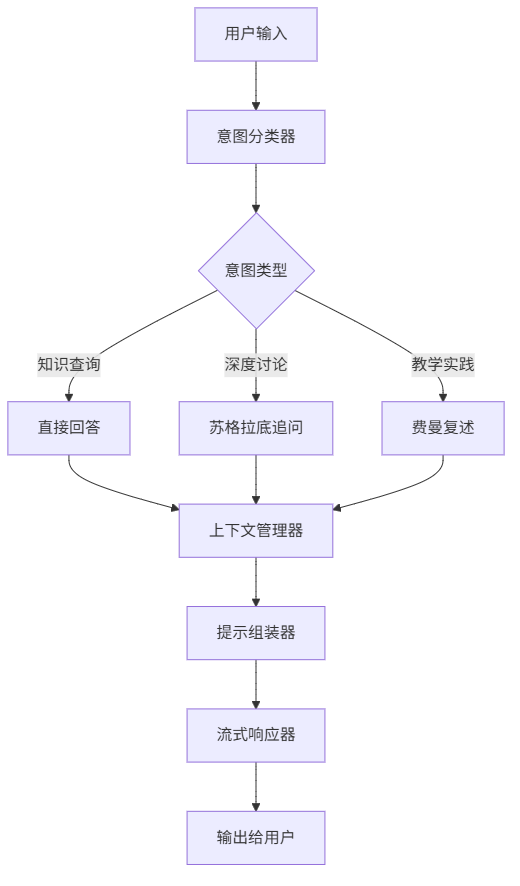
\includegraphics[keepaspectratio,alt={流程图1}]{figures/mermaid-00-38080538.png}}
\caption{流程图1}
\end{figure}

\begin{quote}
注：意图分类器在本地执行（1-5ms），上下文管理器按优先级加载五个维度的上下文。
\end{quote}

\subsection{二、相关工作}\label{ux4e8cux76f8ux5173ux5de5ux4f5c}

\subsubsection{2.1
大语言模型应用架构}\label{ux5927ux8bedux8a00ux6a21ux578bux5e94ux7528ux67b6ux6784}

当前主流的 LLM
应用架构可分为三类：直接调用型、检索增强生成型（RAG{[}3{]}）和智能体编排型{[}4{]}。

\subsubsection{2.2
教学策略驱动的对话系统}\label{ux6559ux5b66ux7b56ux7565ux9a71ux52a8ux7684ux5bf9ux8bddux7cfbux7edf}

教学策略驱动的对话系统借鉴了教育心理学中的 \textbf{Bloom
认知层级理论}{[}5{]}。Bloom 将认知能力分为六个层级，其升降级机制如下：

\begin{figure}
\centering
\pandocbounded{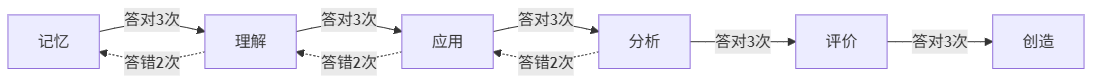
\includegraphics[keepaspectratio,alt={流程图2}]{figures/mermaid-01-4d53823c.png}}
\caption{流程图2}
\end{figure}

\begin{quote}
注：Bloom 层级达到 4 级以上时自动切换苏格拉底追问模式，2
级以下切换为直接回答模式。
\end{quote}

\subsection{三、系统架构设计}\label{ux4e09ux7cfbux7edfux67b6ux6784ux8bbeux8ba1}

\subsubsection{3.1
六步编排流水线}\label{ux516dux6b65ux7f16ux6392ux6d41ux6c34ux7ebf}

六步编排流水线是本系统的核心，每一步的设计目标与延迟分布见表 1。

\begin{quote}
\textbf{表1：六步编排流水线步骤详情与性能画像}
\end{quote}

\begin{table}[htbp]
\centering
\begin{tabularx}{\textwidth}{>{\hsize=0.281\hsize\linewidth=\hsize\raggedright\arraybackslash}X>{\hsize=0.842\hsize\linewidth=\hsize\raggedright\arraybackslash}X>{\hsize=2.175\hsize\linewidth=\hsize\raggedright\arraybackslash}X>{\hsize=0.702\hsize\linewidth=\hsize\raggedright\arraybackslash}X}
\toprule
\textbf{步骤} & \textbf{模块名称} & \textbf{功能描述} & \textbf{平均延迟} \\
\midrule
① & 意图分类器 & 本地关键词打分，识别4类用户意图 & 1-5ms \\
② & 策略选择器 & 意图到教学模式的映射决策 & \textless1ms \\
③ & 状态追踪器 & Bloom层级自适应升降级 & \textless1ms \\
④ & 上下文管理器 & 5维上下文预算制懒加载 & 50-200ms \\
⑤ & 提示组装器 & 四段动态系统提示拼装 & \textless1ms \\
⑥ & 流式响应器 & AI SDK流式输出+归一化 & 500-2000ms \\
\bottomrule
\end{tabularx}
\end{table}

\begin{quote}
注：步骤①-⑤全部在本地执行，合计延迟
52-207ms。步骤⑥为唯一涉及网络请求的环节{[}6{]}。
\end{quote}

\subsubsection{3.2 数学模型}\label{ux6570ux5b66ux6a21ux578b}

渐进式通道压缩策略的核心公式如下：

\[
C_i = C_0 \cdot \alpha^i
\]

\begin{quote}
式(1)：渐进式通道压缩公式
\end{quote}

注意力模块中使用的 Sigmoid 激活函数定义为：

\[
\sigma(x) = \frac{1}{1 + e^{-x}}
\]

\begin{quote}
式(2)：Sigmoid 激活函数
\end{quote}

\subsection{四、实验结果}\label{ux56dbux5b9eux9a8cux7ed3ux679c}

\subsubsection{4.1 Token 消耗对比}\label{token-ux6d88ux8017ux5bf9ux6bd4}

\begin{quote}
\textbf{表2：Token 消耗对比（50 次中等复杂度对话）}
\end{quote}

\begin{table}[htbp]
\centering
\begin{tabularx}{\textwidth}{>{\hsize=1.200\hsize\linewidth=\hsize\raggedright\arraybackslash}X>{\hsize=0.800\hsize\linewidth=\hsize\raggedright\arraybackslash}X>{\hsize=1.200\hsize\linewidth=\hsize\raggedright\arraybackslash}X>{\hsize=0.800\hsize\linewidth=\hsize\raggedright\arraybackslash}X}
\toprule
\textbf{指标} & \textbf{全量加载} & \textbf{预算制懒加载} & \textbf{节省比例} \\
\midrule
平均 Token/次 & 4,200 & 2,600 & 38\% \\
中位 Token/次 & 3,800 & 2,356 & 38\% \\
最大 Token/次 & 6,500 & 2,925 & 55\% \\
\bottomrule
\end{tabularx}
\end{table}

\begin{quote}
注：本方案平均节省 Token 38\%（中位数），最高节省 55\%。
\end{quote}

\subsection{五、结论与展望}\label{ux4e94ux7ed3ux8bbaux4e0eux5c55ux671b}

本文提出了一种基于六步编排流水线的智能体架构，通过预算制懒加载的上下文构建器和
Bloom 认知层级驱动的难度自适应机制，在保持回答质量的同时显著降低了 Token
消耗。

未来的工作将聚焦三个方向：（一）扩展上下文构建器维度；（二）探索基于强化学习的策略自动优化机制{[}1{]}；（三）将架构推广到多模态交互场景。

\subsection{参考文献}\label{ux53c2ux8003ux6587ux732e}

{[}1{]} Brown T, Mann B, Ryder N, et al.~Language models are few-shot
learners{[}C{]}. NeurIPS, 2020. {[}2{]} Yao S, Zhao J, Yu D, et
al.~ReAct: Synergizing reasoning and acting in language models{[}C{]}.
ICLR, 2023. {[}3{]} Lewis P, Perez E, Piktus A, et
al.~Retrieval-augmented generation for knowledge-intensive NLP
tasks{[}C{]}. NeurIPS, 2020. {[}4{]} Wang L, Ma C, Feng X, et al.~A
survey on large language model based autonomous agents{[}J{]}.
arXiv:2308.11432, 2023. {[}5{]} Bloom B S. Taxonomy of educational
objectives{[}M{]}. New York: David McKay, 1956. {[}6{]} Vaswani A,
Shazeer N, Parmar N, et al.~Attention is all you need{[}C{]}. NeurIPS,
2017.

\end{document}
